\documentclass{standalone}
\usepackage{tikz}
\usetikzlibrary{patterns, positioning}
\usepackage[sfdefault]{ClearSans} %% option 'sfdefault' activates Clear Sans as the default text font
\usepackage[T1]{fontenc}

\begin{document}
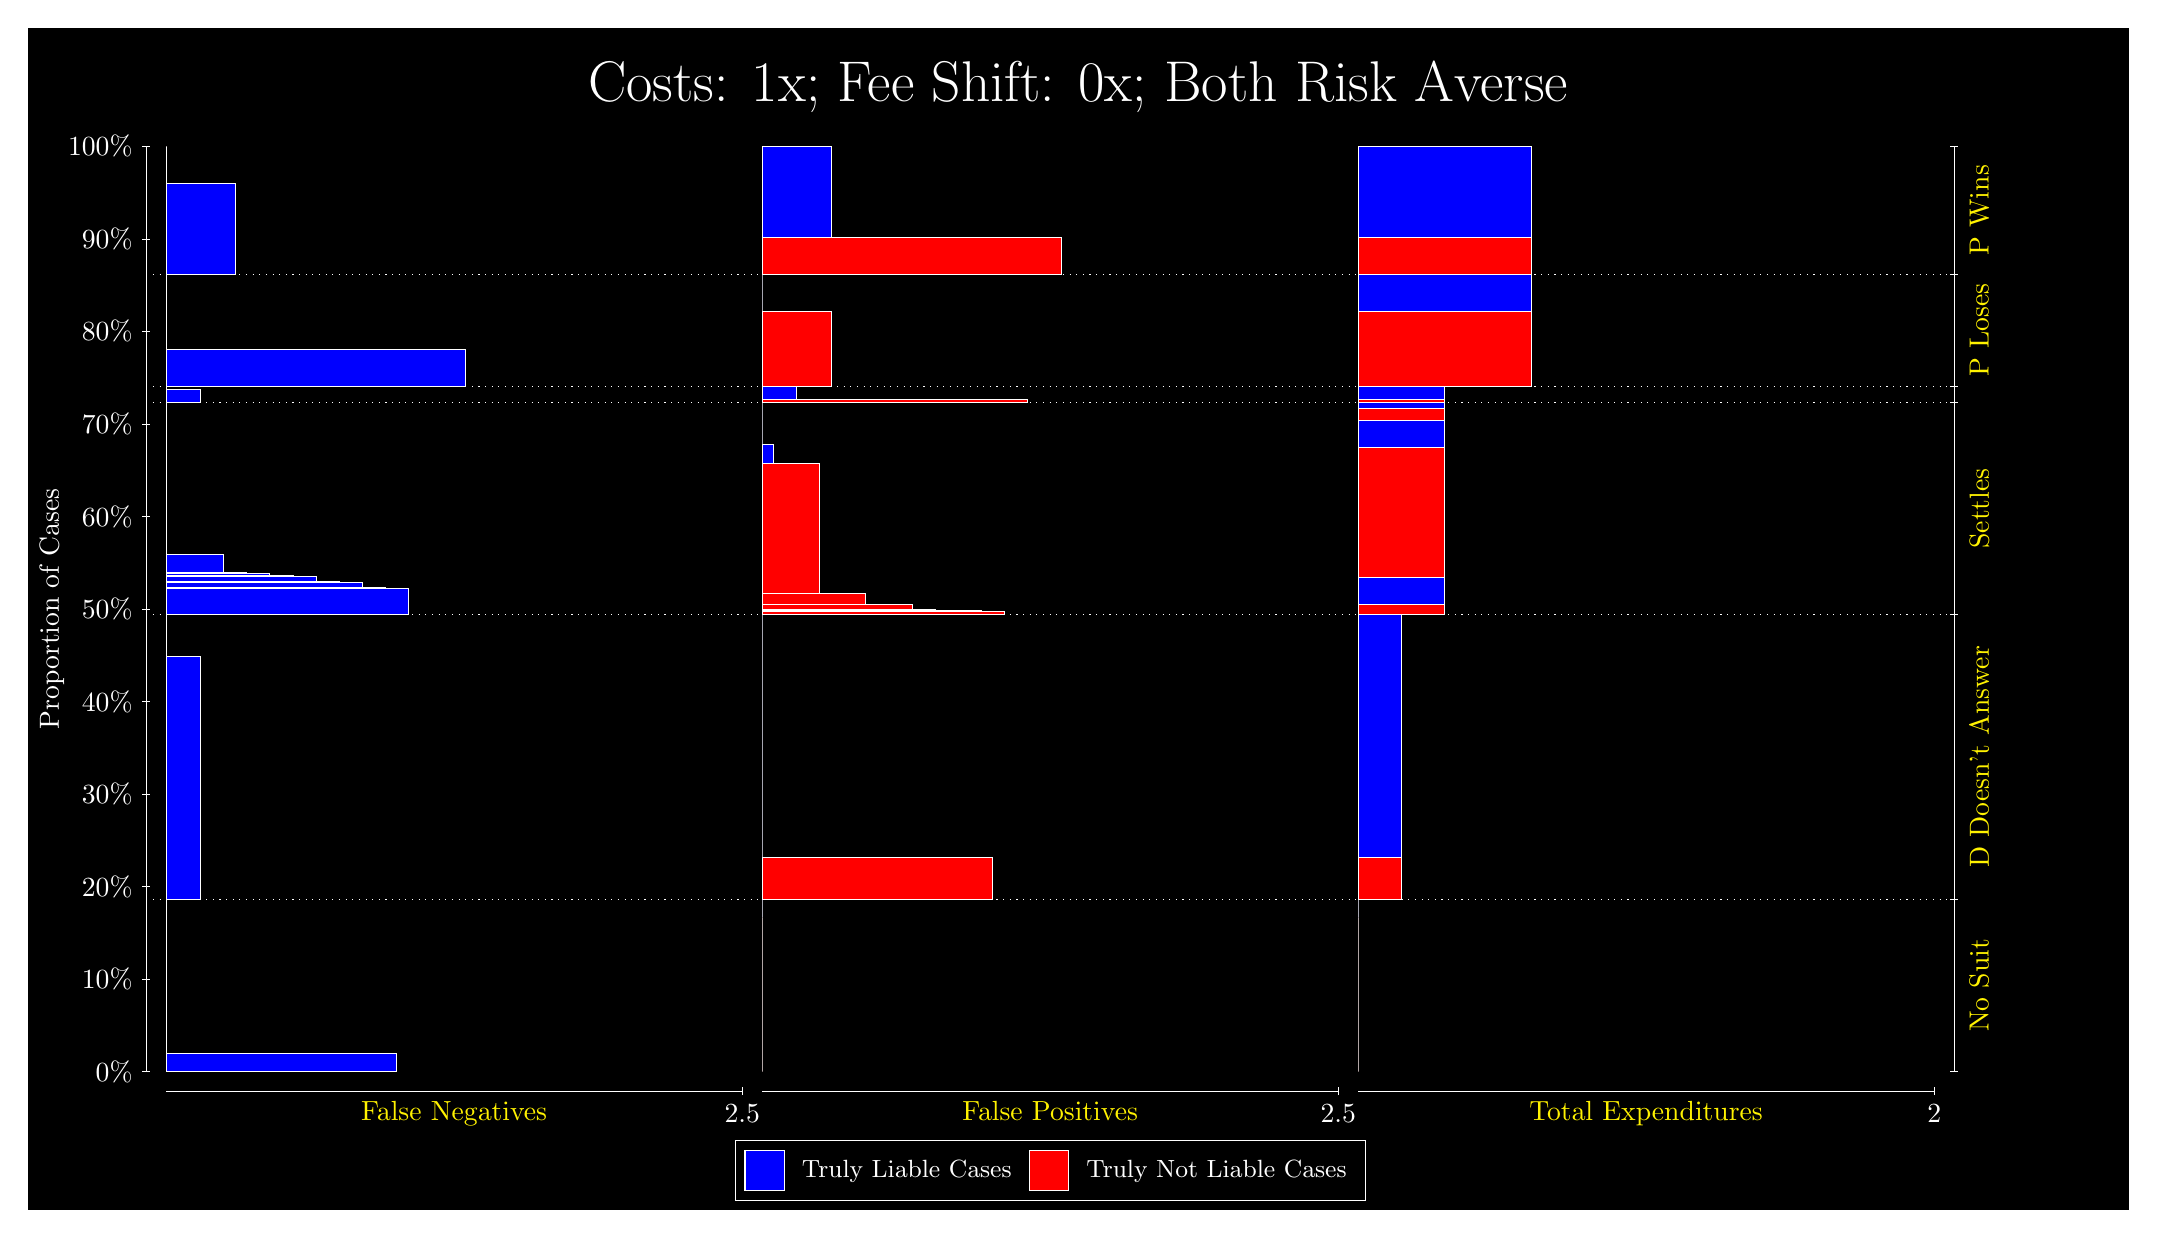
\begin{tikzpicture}
\draw[fill=black] (0,0) rectangle (26.667,15);
\draw[text=white] (0,13.5) rectangle (26.667,15) node[midway] {\huge Costs: 1x; Fee Shift: 0x; Both Risk Averse};
\draw[white, very thin] (1.5,1.75) -- (1.5,13.5);
\node[rotate=90, text=white, anchor=center] at (0.3, 7.625) {Proportion of Cases};
\draw[white, very thin] (1.45,1.75) -- (1.55,1.75);
\node[text=white, anchor=east] at (1.45, 1.75) {0\%};
\draw[white, very thin] (1.45,2.925) -- (1.55,2.925);
\node[text=white, anchor=east] at (1.45, 2.925) {10\%};
\draw[white, very thin] (1.45,4.1) -- (1.55,4.1);
\node[text=white, anchor=east] at (1.45, 4.1) {20\%};
\draw[white, very thin] (1.45,5.275) -- (1.55,5.275);
\node[text=white, anchor=east] at (1.45, 5.275) {30\%};
\draw[white, very thin] (1.45,6.45) -- (1.55,6.45);
\node[text=white, anchor=east] at (1.45, 6.45) {40\%};
\draw[white, very thin] (1.45,7.625) -- (1.55,7.625);
\node[text=white, anchor=east] at (1.45, 7.625) {50\%};
\draw[white, very thin] (1.45,8.8) -- (1.55,8.8);
\node[text=white, anchor=east] at (1.45, 8.8) {60\%};
\draw[white, very thin] (1.45,9.975) -- (1.55,9.975);
\node[text=white, anchor=east] at (1.45, 9.975) {70\%};
\draw[white, very thin] (1.45,11.15) -- (1.55,11.15);
\node[text=white, anchor=east] at (1.45, 11.15) {80\%};
\draw[white, very thin] (1.45,12.325) -- (1.55,12.325);
\node[text=white, anchor=east] at (1.45, 12.325) {90\%};
\draw[white, very thin] (1.45,13.5) -- (1.55,13.5);
\node[text=white, anchor=east] at (1.45, 13.5) {100\%};

\draw[white, very thin] (24.457,1.75) -- (24.457,13.5);
\draw[white, very thin] (24.407,1.75) -- (24.507,1.75);
\node[anchor=west] at (24.407, 1.75) {};
\draw[white, very thin] (24.407,3.9363) -- (24.507,3.9363);
\node[anchor=west] at (24.407, 3.9363) {};
\draw[white, very thin] (24.407,7.5524) -- (24.507,7.5524);
\node[anchor=west] at (24.407, 7.5524) {};
\draw[white, very thin] (24.407,10.249) -- (24.507,10.249);
\node[anchor=west] at (24.407, 10.249) {};
\draw[white, very thin] (24.407,10.452) -- (24.507,10.452);
\node[anchor=west] at (24.407, 10.452) {};
\draw[white, very thin] (24.407,11.877) -- (24.507,11.877);
\node[anchor=west] at (24.407, 11.877) {};
\draw[white, very thin] (24.407,13.5) -- (24.507,13.5);
\node[anchor=west] at (24.407, 13.5) {};

\draw[white, very thin, fill=blue] (1.75,1.75) rectangle (4.6775,1.98);
\draw[white, very thin, fill=red] (1.75,1.98) rectangle (1.75,3.9363);
\draw[white, very thin, fill=blue] (1.75,3.9363) rectangle (2.1891,7.0203);
\draw[white, very thin, fill=red] (1.75,7.0203) rectangle (1.75,7.5524);
\draw[white, very thin, fill=blue] (1.75,7.5524) rectangle (4.8239,7.8933);
\draw[white, very thin, fill=blue] (1.75,7.8933) rectangle (4.5312,7.901);
\draw[white, very thin, fill=blue] (1.75,7.901) rectangle (4.2384,7.9657);
\draw[white, very thin, fill=blue] (1.75,7.9657) rectangle (3.9457,7.974);
\draw[white, very thin, fill=blue] (1.75,7.974) rectangle (3.6529,8.0416);
\draw[white, very thin, fill=blue] (1.75,8.0416) rectangle (3.3602,8.0508);
\draw[white, very thin, fill=blue] (1.75,8.0508) rectangle (3.0674,8.0763);
\draw[white, very thin, fill=blue] (1.75,8.0763) rectangle (2.7746,8.0861);
\draw[white, very thin, fill=blue] (1.75,8.0861) rectangle (2.4819,8.3227);
\draw[white, very thin, fill=red] (1.75,8.3227) rectangle (1.75,10.249);
\draw[white, very thin, fill=blue] (1.75,10.249) rectangle (2.1891,10.417);
\draw[white, very thin, fill=red] (1.75,10.417) rectangle (1.75,10.452);
\draw[white, very thin, fill=blue] (1.75,10.452) rectangle (5.5558,10.917);
\draw[white, very thin, fill=red] (1.75,10.917) rectangle (1.75,11.877);
\draw[white, very thin, fill=blue] (1.75,11.877) rectangle (2.6283,13.034);
\draw[white, very thin, fill=red] (1.75,13.034) rectangle (1.75,13.5);
\draw[white, very thin, fill=red] (9.3189,1.75) rectangle (9.3189,3.7063);
\draw[white, very thin, fill=blue] (9.3189,3.7063) rectangle (9.3189,3.9363);
\draw[white, very thin, fill=red] (9.3189,3.9363) rectangle (12.246,4.4684);
\draw[white, very thin, fill=blue] (9.3189,4.4684) rectangle (9.3189,7.5524);
\draw[white, very thin, fill=red] (9.3189,7.5524) rectangle (12.393,7.5975);
\draw[white, very thin, fill=red] (9.3189,7.5975) rectangle (12.1,7.6019);
\draw[white, very thin, fill=red] (9.3189,7.6019) rectangle (11.807,7.6135);
\draw[white, very thin, fill=red] (9.3189,7.6135) rectangle (11.515,7.6176);
\draw[white, very thin, fill=red] (9.3189,7.6176) rectangle (11.222,7.6804);
\draw[white, very thin, fill=red] (9.3189,7.6804) rectangle (10.929,7.6887);
\draw[white, very thin, fill=red] (9.3189,7.6887) rectangle (10.636,7.8218);
\draw[white, very thin, fill=red] (9.3189,7.8218) rectangle (10.344,7.8296);
\draw[white, very thin, fill=red] (9.3189,7.8296) rectangle (10.051,9.4782);
\draw[white, very thin, fill=blue] (9.3189,9.4782) rectangle (9.4652,9.7148);
\draw[white, very thin, fill=blue] (9.3189,9.7148) rectangle (9.3189,10.249);
\draw[white, very thin, fill=red] (9.3189,10.249) rectangle (12.686,10.284);
\draw[white, very thin, fill=blue] (9.3189,10.284) rectangle (9.758,10.452);
\draw[white, very thin, fill=red] (9.3189,10.452) rectangle (10.197,11.411);
\draw[white, very thin, fill=blue] (9.3189,11.411) rectangle (9.3189,11.877);
\draw[white, very thin, fill=red] (9.3189,11.877) rectangle (13.125,12.343);
\draw[white, very thin, fill=blue] (9.3189,12.343) rectangle (10.197,13.5);
\draw[white, very thin, fill=red] (16.888,1.75) rectangle (16.888,3.7063);
\draw[white, very thin, fill=blue] (16.888,3.7063) rectangle (16.888,3.9363);
\draw[white, very thin, fill=red] (16.888,3.9363) rectangle (17.437,4.4684);
\draw[white, very thin, fill=blue] (16.888,4.4684) rectangle (17.437,7.5524);
\draw[white, very thin, fill=red] (16.888,7.5524) rectangle (17.986,7.6804);
\draw[white, very thin, fill=blue] (16.888,7.6804) rectangle (17.986,8.0292);
\draw[white, very thin, fill=red] (16.888,8.0292) rectangle (17.986,9.6779);
\draw[white, very thin, fill=blue] (16.888,9.6779) rectangle (17.986,10.019);
\draw[white, very thin, fill=red] (16.888,10.019) rectangle (17.986,10.168);
\draw[white, very thin, fill=blue] (16.888,10.168) rectangle (17.986,10.249);
\draw[white, very thin, fill=red] (16.888,10.249) rectangle (17.986,10.284);
\draw[white, very thin, fill=blue] (16.888,10.284) rectangle (17.986,10.452);
\draw[white, very thin, fill=red] (16.888,10.452) rectangle (19.083,11.411);
\draw[white, very thin, fill=blue] (16.888,11.411) rectangle (19.083,11.877);
\draw[white, very thin, fill=red] (16.888,11.877) rectangle (19.083,12.343);
\draw[white, very thin, fill=blue] (16.888,12.343) rectangle (19.083,13.5);
\draw[white, dotted] (1.5,3.9363) -- (24.457,3.9363);
\draw[white, dotted] (1.5,7.5524) -- (24.457,7.5524);
\draw[white, dotted] (1.5,10.249) -- (24.457,10.249);
\draw[white, dotted] (1.5,10.452) -- (24.457,10.452);
\draw[white, dotted] (1.5,11.877) -- (24.457,11.877);
\draw[white, very thin] (1.75,1.5) -- (9.0689,1.5);
\node[text=yellow, anchor=north] at (5.4094, 1.5) {False Negatives};
\draw[white, very thin] (9.0689,1.45) -- (9.0689,1.55);
\node[text=white, anchor=north] at (9.0689, 1.45) {2.5};

\draw[white, very thin] (9.3189,1.5) -- (16.638,1.5);
\node[text=yellow, anchor=north] at (12.978, 1.5) {False Positives};
\draw[white, very thin] (16.638,1.45) -- (16.638,1.55);
\node[text=white, anchor=north] at (16.638, 1.45) {2.5};

\draw[white, very thin] (16.888,1.5) -- (24.207,1.5);
\node[text=yellow, anchor=north] at (20.547, 1.5) {Total Expenditures};
\draw[white, very thin] (24.207,1.45) -- (24.207,1.55);
\node[text=white, anchor=north] at (24.207, 1.45) {2};

\node[text=yellow, centered, rotate=90] at (24.777, 2.8432) {No Suit};
\node[text=yellow, centered, rotate=90] at (24.777, 5.7444) {D Doesn't Answer};
\node[text=yellow, centered, rotate=90] at (24.777, 8.9005) {Settles};

\node[text=yellow, centered, rotate=90] at (24.777, 11.164) {P Loses};
\node[text=yellow, centered, rotate=90] at (24.777, 12.688) {P Wins};

\draw (12.978300999999998,1.5) node[draw=none] (baseCoordinate) {};
\begin{scope}[align=center]
        \matrix[scale=0.5, draw=white, below=0.5cm of baseCoordinate, nodes={draw}, column sep=0.1cm]{
            \node[rectangle, draw, minimum width=0.5cm, minimum height=0.5cm, fill=blue] {}; &
            \node[draw=none, font=\small, text=white] (B) {Truly Liable Cases}; &
            \node[rectangle, draw, minimum width=0.5cm, minimum height=0.5cm, fill=red] {}; &
            \node[draw=none, font=\small, text=white] (B) {Truly Not Liable Cases}; \\
            };
\end{scope}

\end{tikzpicture}
\end{document}